\documentclass[11pt]{article}


    \usepackage[breakable]{tcolorbox}
    \tcbset{nobeforeafter} % prevents tcolorboxes being placing in paragraphs
    \usepackage{float}
    \floatplacement{figure}{H} % forces figures to be placed at the correct location
    \usepackage{multicol}
	\usepackage[english]{babel}
    \usepackage{tabularx}
    \usepackage{subfigure}
    \usepackage{picture}
    \usepackage{amsmath}
    \usepackage{hyperref}
    \hypersetup{
    colorlinks=true,
    linkcolor=blue,
    filecolor=magenta,      
    urlcolor=cyan,
    }
    \usepackage{graphicx}    
    \usepackage{caption}
    \usepackage{adjustbox} % Used to constrain images to a maximum size 
    \usepackage{xcolor} % Allow colors to be defined
    \usepackage{enumerate} % Needed for markdown enumerations to work
    \usepackage{geometry} % Used to adjust the document margins
    \usepackage{amsmath} % Equations
    \usepackage{amssymb} % Equations
    \definecolor{urlcolor}{rgb}{0,.145,.698}
    \definecolor{linkcolor}{rgb}{.71,0.21,0.01}
    \definecolor{citecolor}{rgb}{.12,.54,.11}
    

    
    % Prevent overflowing lines due to hard-to-break entities
    \sloppy 
    % Setup hyperref package
    \hypersetup{
      breaklinks=true,  % so long urls are correctly broken across lines
      colorlinks=true,
      urlcolor=urlcolor,
      linkcolor=linkcolor,
      citecolor=citecolor,
      }
    % Slightly bigger margins than the latex defaults
    
    \geometry{verbose,tmargin=1in,bmargin=1in,lmargin=0.6in,rmargin=0.6in}
    \usepackage{fancyhdr}
    \pagestyle{fancy}
    \renewcommand{\footrulewidth}{1pt}
    \rhead{e12045110 , e12045110, e11921655}
    \lhead{VU\,184.702\\ Machine Learning}
    \cfoot{\thepage}
    \setcounter{secnumdepth}{0}
    \setlength\parindent{0pt}

    \usepackage{booktabs}

    \usepackage{listings}
    \usepackage[linesnumbered,ruled,vlined]{algorithm2e}
    \newcommand\mycommfont[1]{\footnotesize\ttfamily\textcolor{blue}{#1}}
    \SetCommentSty{mycommfont}
    \SetKwInput{KwInput}{Input}                % Set the Input
    \SetKwInput{KwOutput}{Output}              % set the Output



\title{Exercise 3}
\author{e11921655 Fabian Holzberger}
\date{\today}

\begin{document}
\graphicspath{{./figures/}}
\maketitle
\section{Part1}

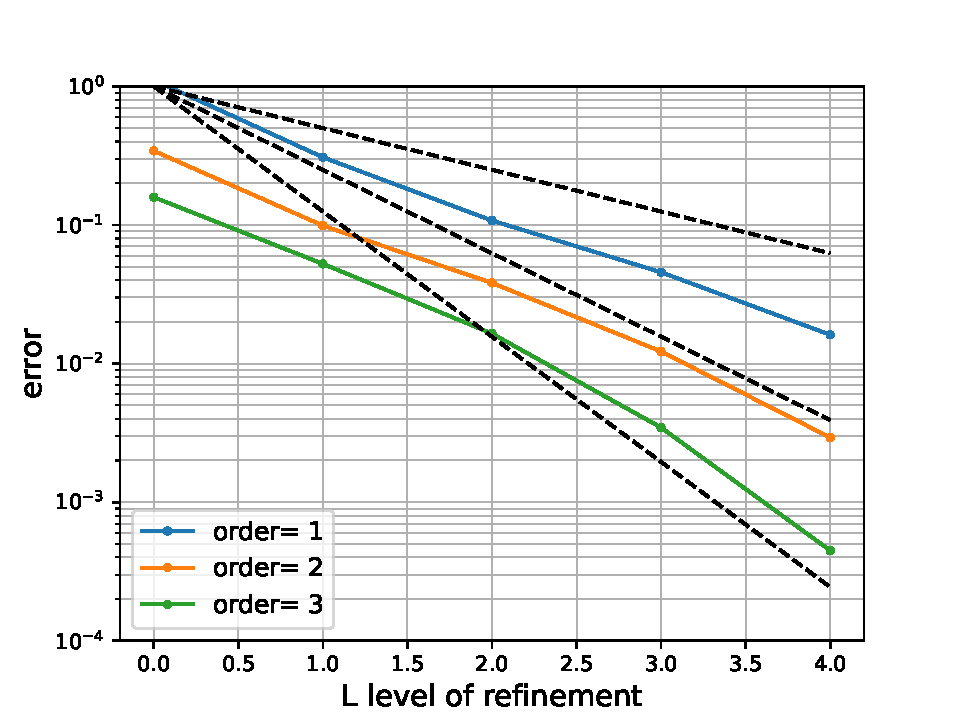
\includegraphics[width=0.7\columnwidth]{norms_ex31.pdf}

\section{Part2}

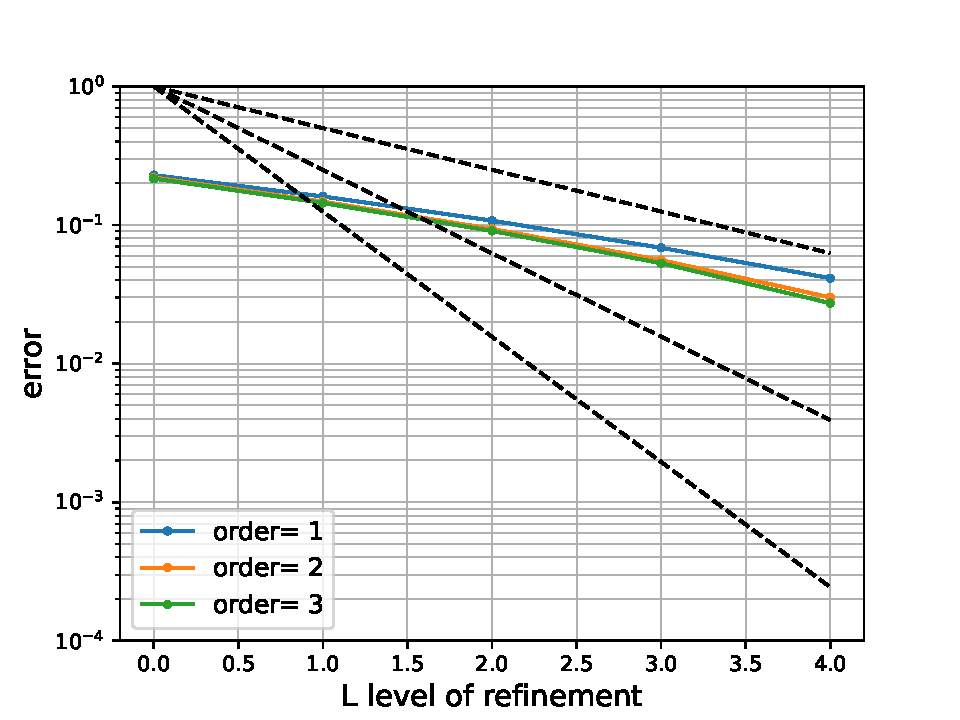
\includegraphics[width=0.7\columnwidth]{norms_ex32.pdf}

\section{Part3}

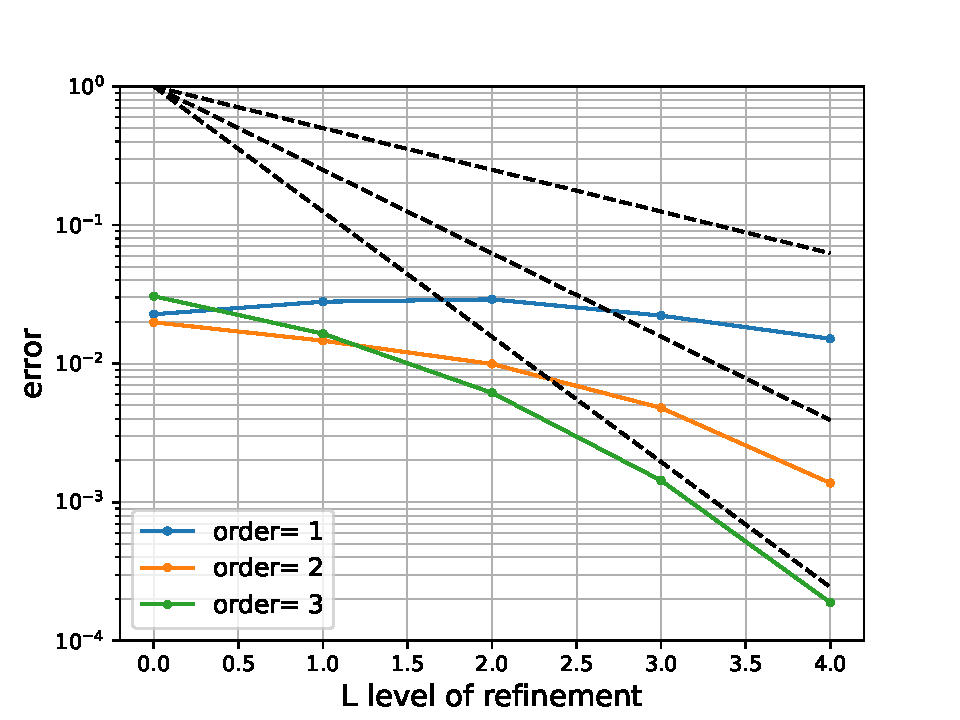
\includegraphics[width=0.7\columnwidth]{norms_ex33.pdf}

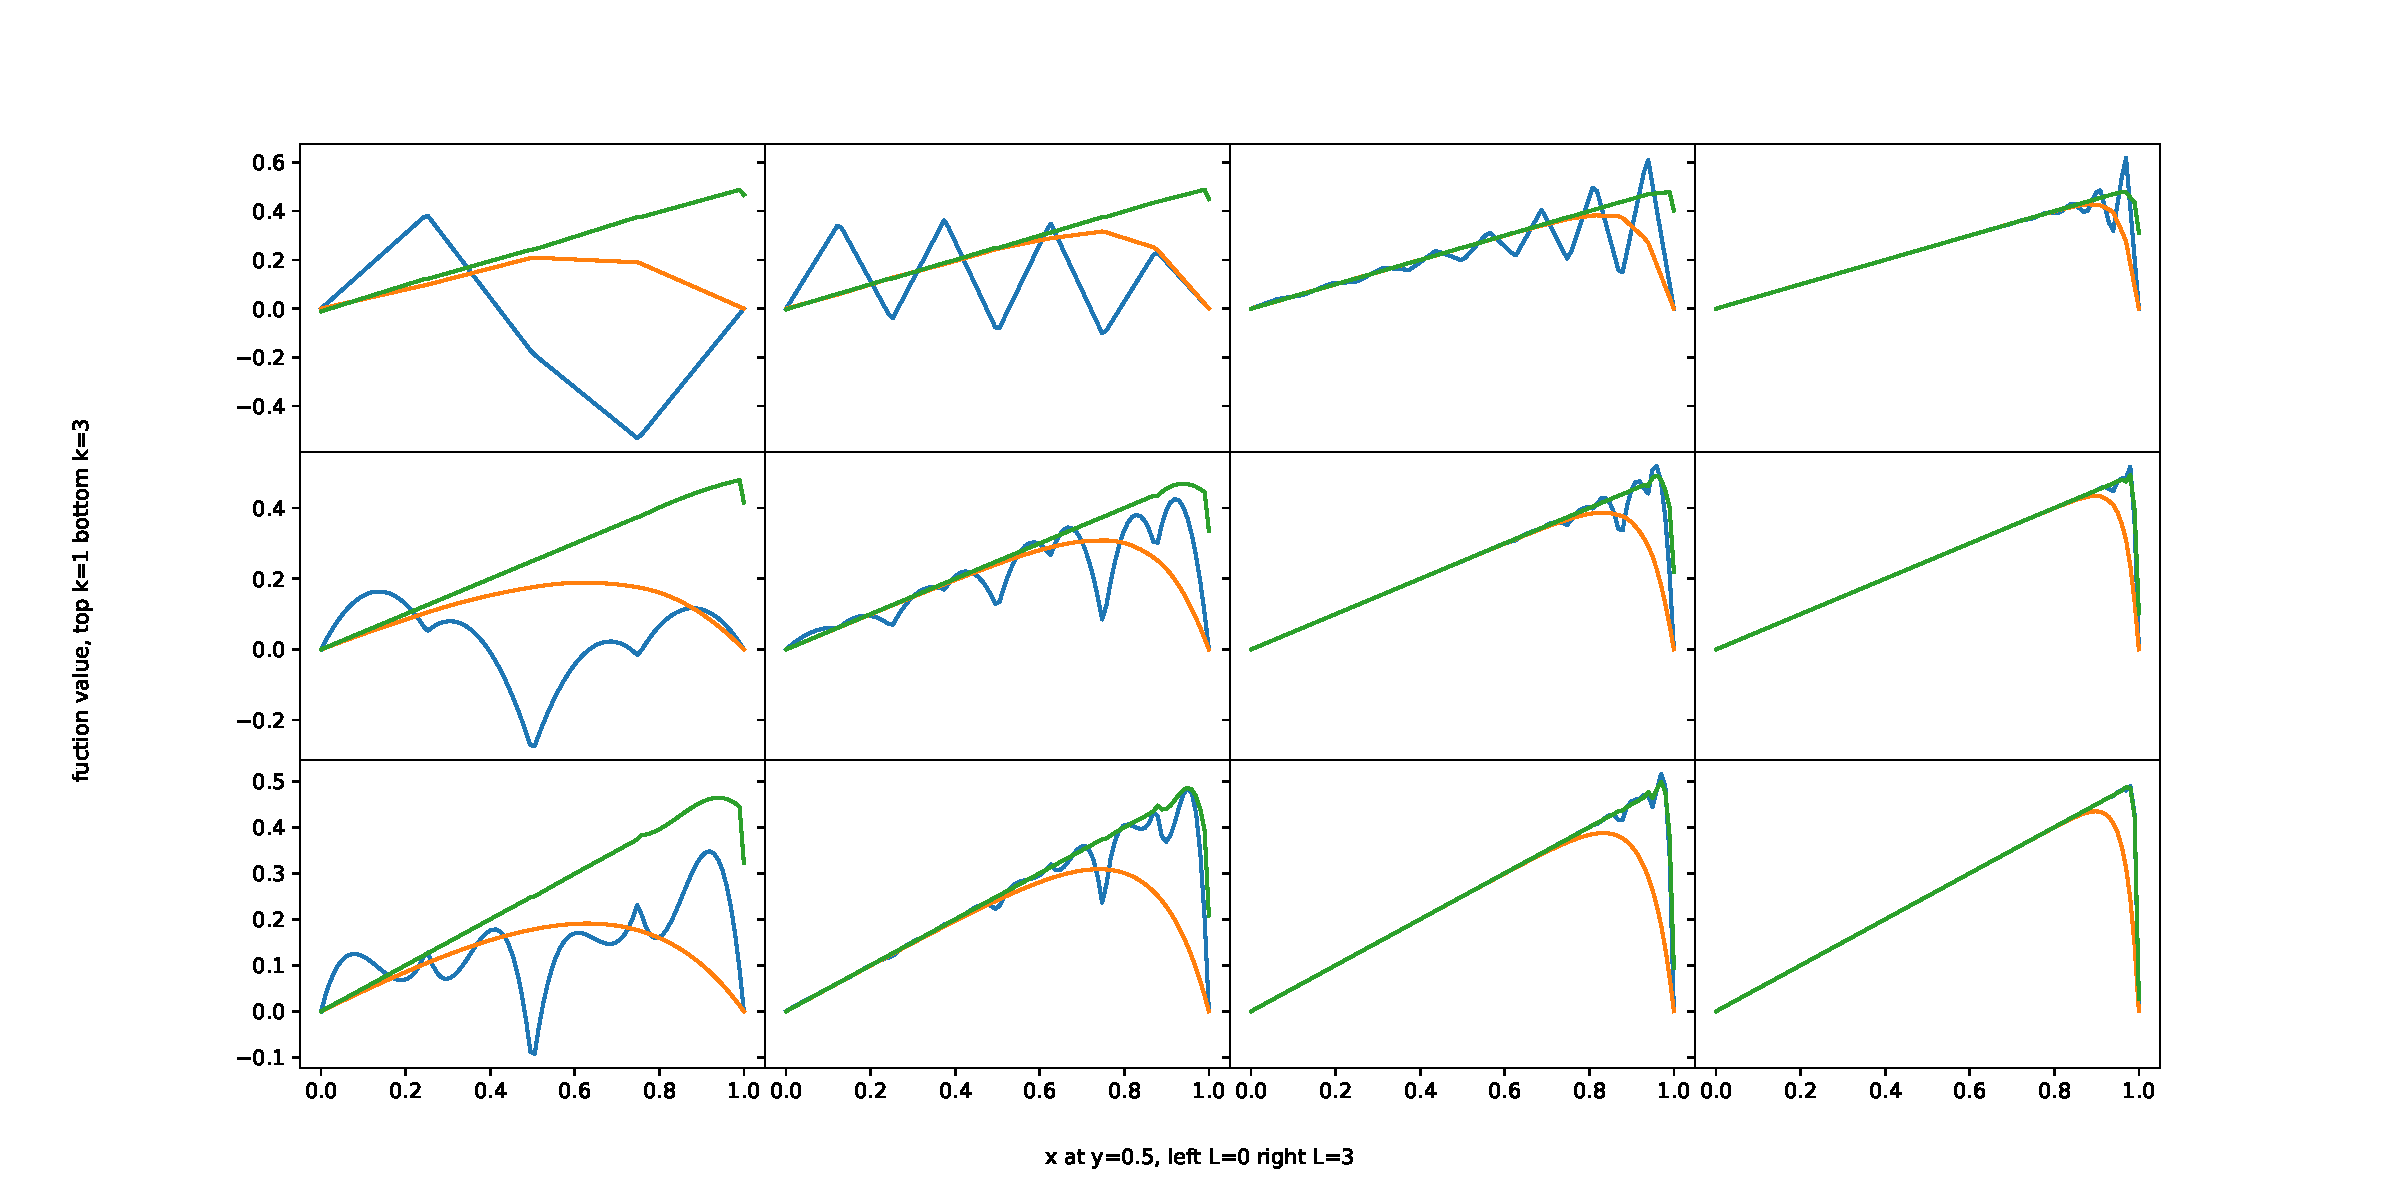
\includegraphics[width=\columnwidth]{cut_ex3_123.pdf}

\section{Part4}

\subsection{solution for $\nu=0.01$ at $L=3$}

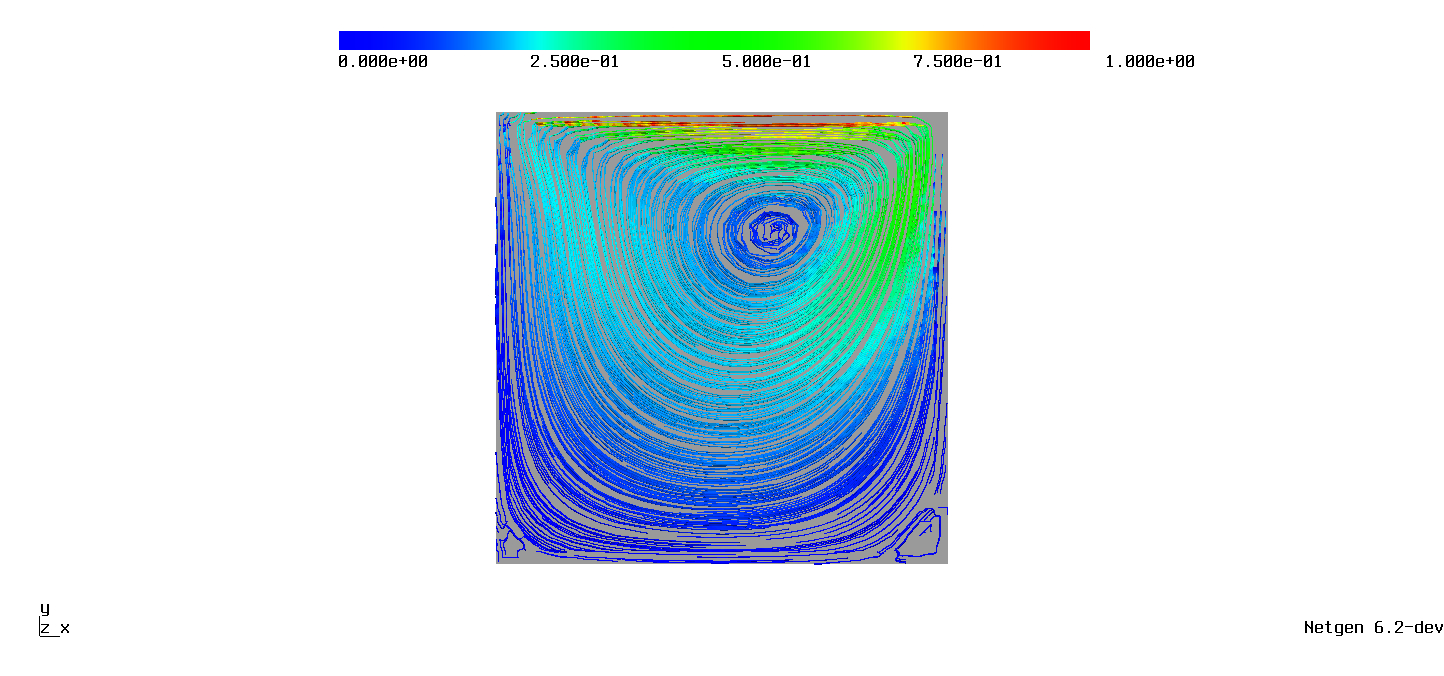
\includegraphics[width=\columnwidth]{ex34_001_stream}


\subsection{solution for $\nu=0.002$ at $L=3$}
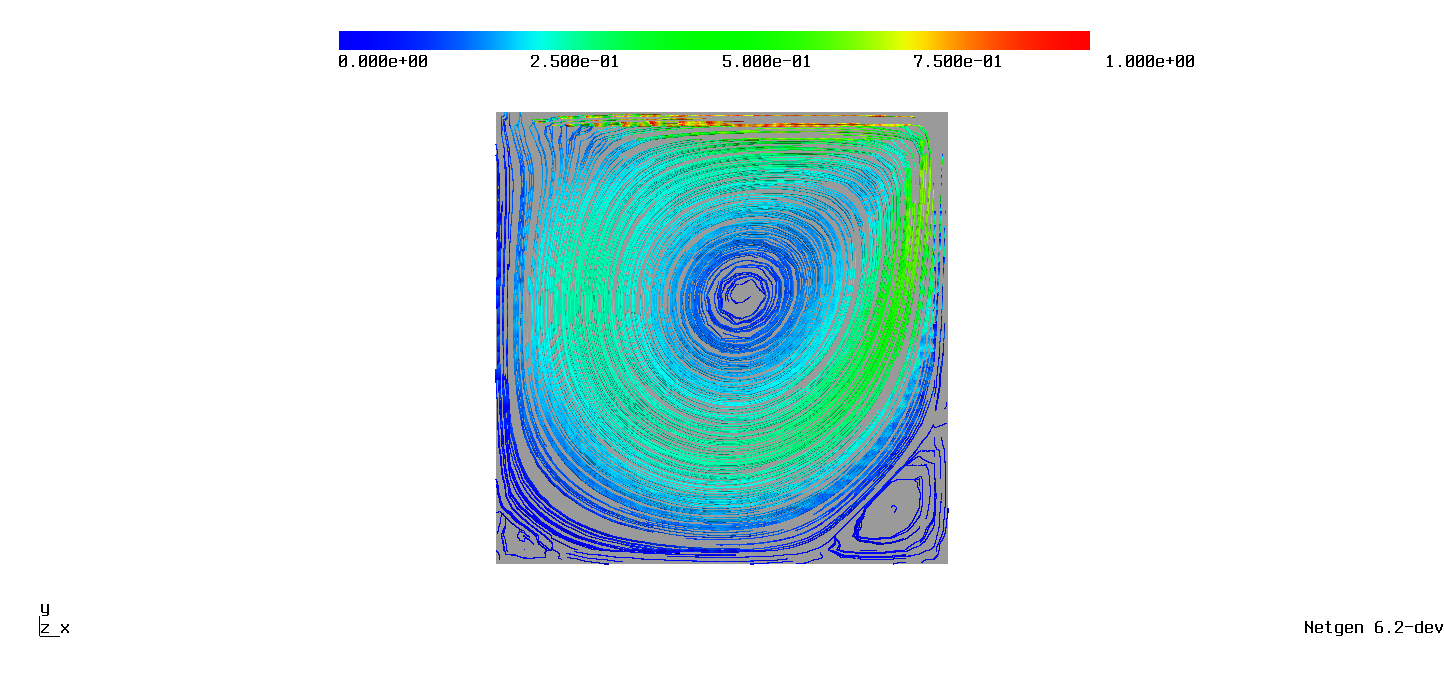
\includegraphics[width=\columnwidth]{ex34_0002_stream}


\subsection{solution for $\nu=0.001$ at $L=3$}
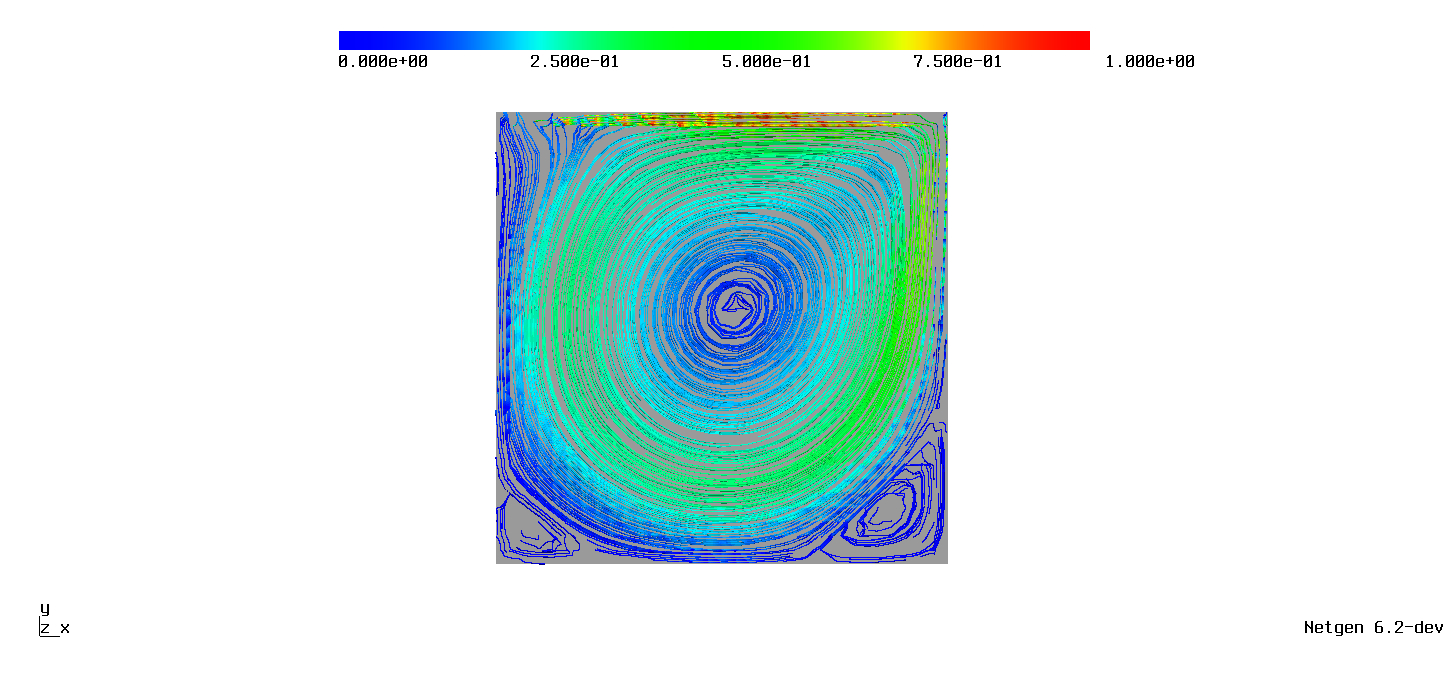
\includegraphics[width=\columnwidth]{ex34_0001_stream}


\subsection{Iterations needed for convergence}

\begin{tabular}{l| l l l l}
	Method, L & 0 &1 &2 &3 \\
	\hline
	$\nu=0.01$\\
	Newton	  & 5 & 5&5 &5\\
	Picard	  & 15 & 16&16 &16\\
	\hline
	$\nu=0.002$\\
	Newton	  & - & 10&8 &8\\
	Picard	  & 79 & 32&34 &34\\
	\hline
	$\nu=0.001$\\
	Newton	  & - & - &- &-\\
	Picard	  & - & 48&37 &38\\
\end{tabular}

\section{Part5}
\subsection{Weak form of NS-equation}
Assume we given the NS-equations in weak form with $(u, p)\in V \times Q=H_0^1(\Omega)^2\times\L_0^2(\Omega)$:
\begin{align}
	(\frac{du}{dt}, v) + a(u, v) + c(u,u,v) + b(v,p) + b(u,q) + \epsilon(p,q) = f(v) \quad \forall (v,q)\in V \times Q
\end{align}
\subsection{Time discretisation by $\theta$-scheme}
\begin{align}
	(u^{n+1}, v) + \theta \tau a(u^{n+1}, v) +& \theta \tau c(u^{n+1},u^{n+1},v) + \tau b(v,p^{n+1}) + \tau b(u^{n+1},q) \tau (p^{n+1},q) =\notag \\ 
	&\tau f(v) + (u^{n}, v) -(1-\theta) \tau a(u^{n}, v) - (1-\theta) \tau c(u^{n},u^{n},v)
\end{align}

Next assume $u_{i+1}^{n+1}=u_i^{n+1} + \delta u_i^{n+1}$ and $p_{i+1}^{n+1}=p_i^{n+1} + \delta p_i^{n+1}$ where $u^{n+1}_0 = u^{n+1}_K$ and  $p^{n+1}_0 = p^{n+1}_K$ for $K\rightarrow \infty$. 
Note further:

\begin{align}
c(u^{n+1}_{i+1},u^{n+1}_{i+1},v) = c(u^{n+1}_{i},\delta u^{n+1}_{i},v) + c(\delta u^{n+1}_{i},u^{n+1}_{i},v) +c(u^{n+1}_{i},u^{n+1}_{i},v) +c(\delta u^{n+1}_{i},\delta u^{n+1}_{i},v)
\end{align}

Then for a Newton method we assume $c(\delta u^{n+1}_{i},\delta u^{n+1}_{i},v)$ and for the picard iteration additionally $c(\delta u^{n+1}_{i},u^{n+1}_{i},v)$.

\subsection{Newton iteration}
\begin{align}
	&(\delta u^{n+1}_i, v) + \theta \tau \left[ a(\delta u^{n+1}_i, v) + c(\delta u^{n+1}_i,u^{n+1}_i,v)+c(u^{n+1}_i,\delta u^{n+1}_i,v) )\right] + \tau\left[ b(v,\delta p^{n+1}_i) + b(\delta u^{n+1}_i,q) + \epsilon (\delta p^{n+1}_i,q)\right] = \notag \\ 
	&(u^{n+1}_0 -u^{n+1}_i , v) + \tau f(v) + (1-\theta) \tau \left[-a(u^{n+1}_0, v) -  c(u^{n+1}_0,u^{n+1}_0,v)\right] 
	+ \theta \tau\left[- a(u^{n+1}_i, v) - c(u^{n+1}_i,u^{n+1}_i,v)\right]\notag \\ 
	&+ \tau\left[-b(v,p^{n+1}_i) - b(u^{n+1}_i,q) - \epsilon (p^{n+1}_i,q) \right]
\end{align}
\subsection{Picard iteration}
\begin{align}
	&(\delta u^{n+1}_i, v) + \theta \tau\left[ c(\delta u^{n+1}_i,u^{n+1}_i,v)+c(u^{n+1}_i,\delta u^{n+1}_i,v) )\right] + \tau\left[ b(v,\delta p^{n+1}_i) + b(\delta u^{n+1}_i,q) + \epsilon (\delta p^{n+1}_i,q)\right] = \notag \\ 
	&(u^{n+1}_0 -u^{n+1}_i , v) + \tau f(v) + (1-\theta) \tau \left[-a(u^{n+1}_0, v) -  c(u^{n+1}_0,u^{n+1}_0,v)\right] 
	+ \theta \tau\left[- a(u^{n+1}_i, v) - c(u^{n+1}_i,u^{n+1}_i,v)\right]\notag \\ 
	&+ \tau\left[-b(v,p^{n+1}_i) - b(u^{n+1}_i,q) - \epsilon (p^{n+1}_i,q) \right]
\end{align}

\subsection{Space discretisation by Tailor-Hood element}
The Taylor-Hood pair of order $k$ is given by:
\begin{align}
	& V_h := \{v \in H_0^1(\Omega)^2:\ v|_T\in P^k(T)^2\quad \forall T\in\mathcal{T}_h \} \notag \\
	& Q_h := \{q \in L_0^2(\Omega)\cap C(\bar{\Omega}):\ q|_T\in P^k(T)\quad \forall T\in\mathcal{T}_h \} \notag \\
\end{align}

\subsection{Mesh}
We choose a trtraheder mesh with 972 Elements and 550 vertices. The global mesh size is 0.05 where the local redinement at the cylinder wall is choosen to be 0.009. The mesh is shown below:
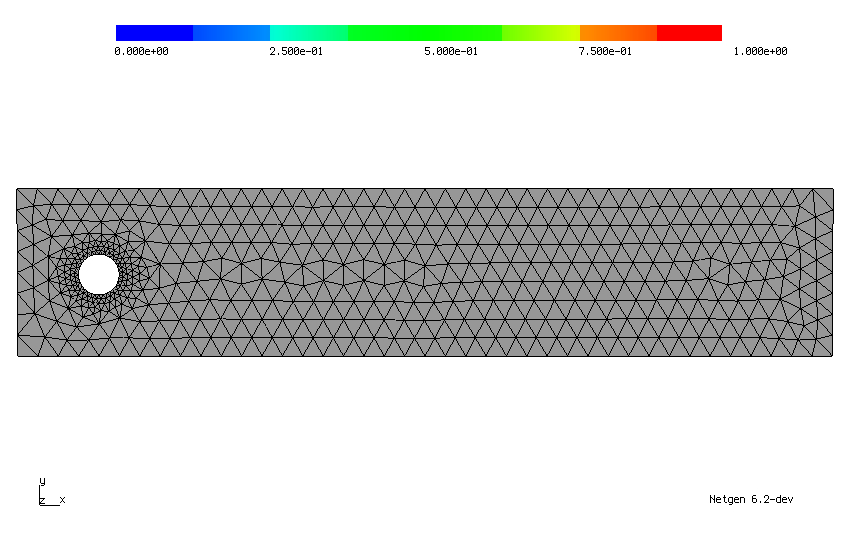
\includegraphics[width=0.7\columnwidth]{mesh35}

To improve the solution quality p-refinements were conducted for different orders $k$ of the Taylor hood space where in contrast to that h-refinements were choosen for the reference solutions. In the Table below we compare cases where h-refinement of the reference and p-refinements of our solution yield a simillar number of free-dofs.

\begin{tabular}{l l l l}
	Lv ref. & order this & free-dofs ref. & free-dofs this\\
	2       & 2	& 2704  & 4221\\
	3       & 3	& 10608 & 10504\\
	-       & 4 	& -	& 19709\\
	4       & 5	& 42016 & 31836\\
	6 	& - 	& 667264& -
\end{tabular}

\subsection{Investigating influence of $\theta$ values on solution for $t\in[0,2]$}

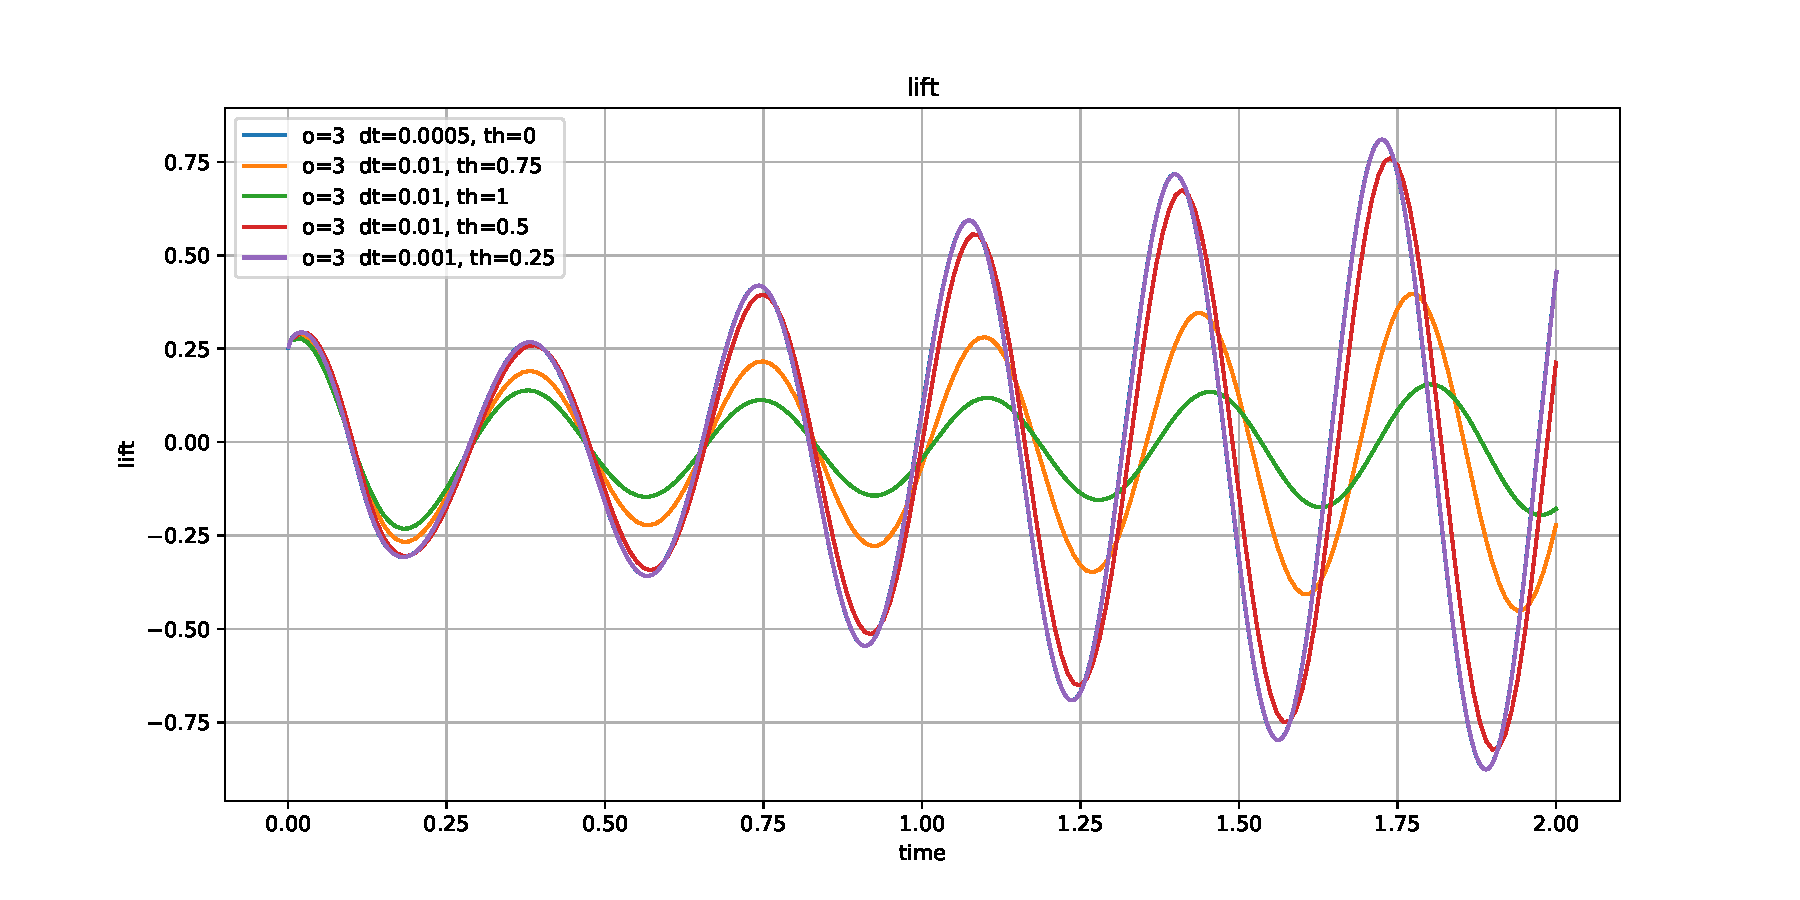
\includegraphics[width=0.75\columnwidth]{lift_full_theta}

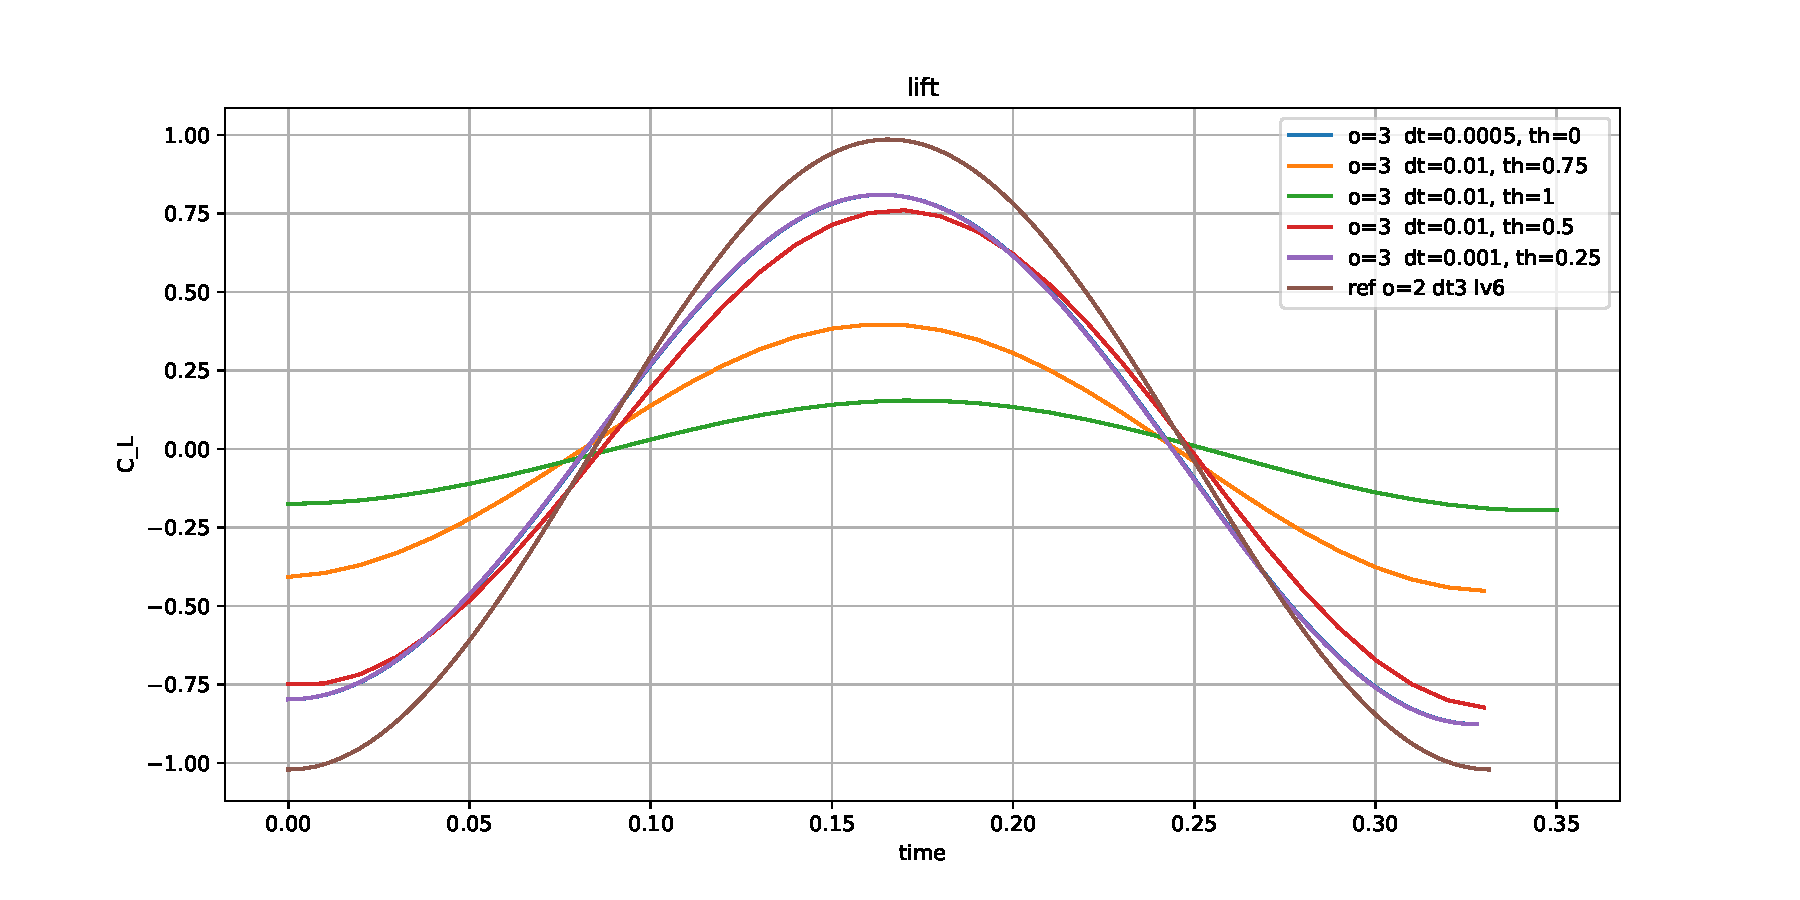
\includegraphics[width=0.75\columnwidth]{lift_theta}

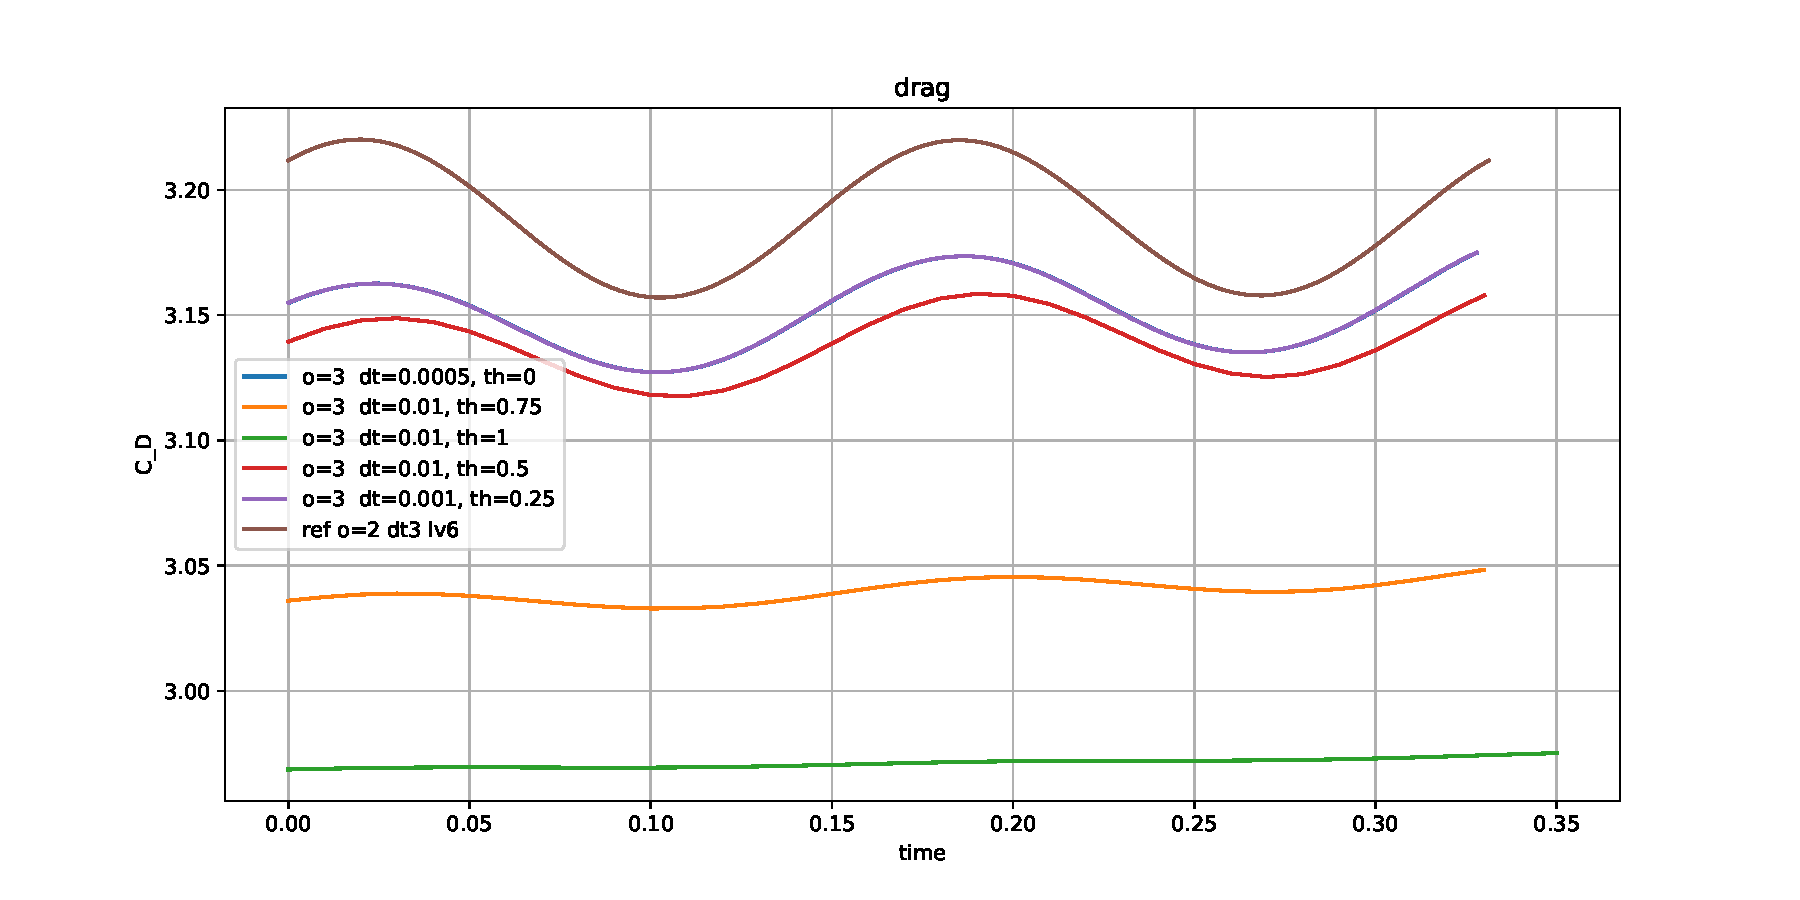
\includegraphics[width=0.75\columnwidth]{drag_theta}

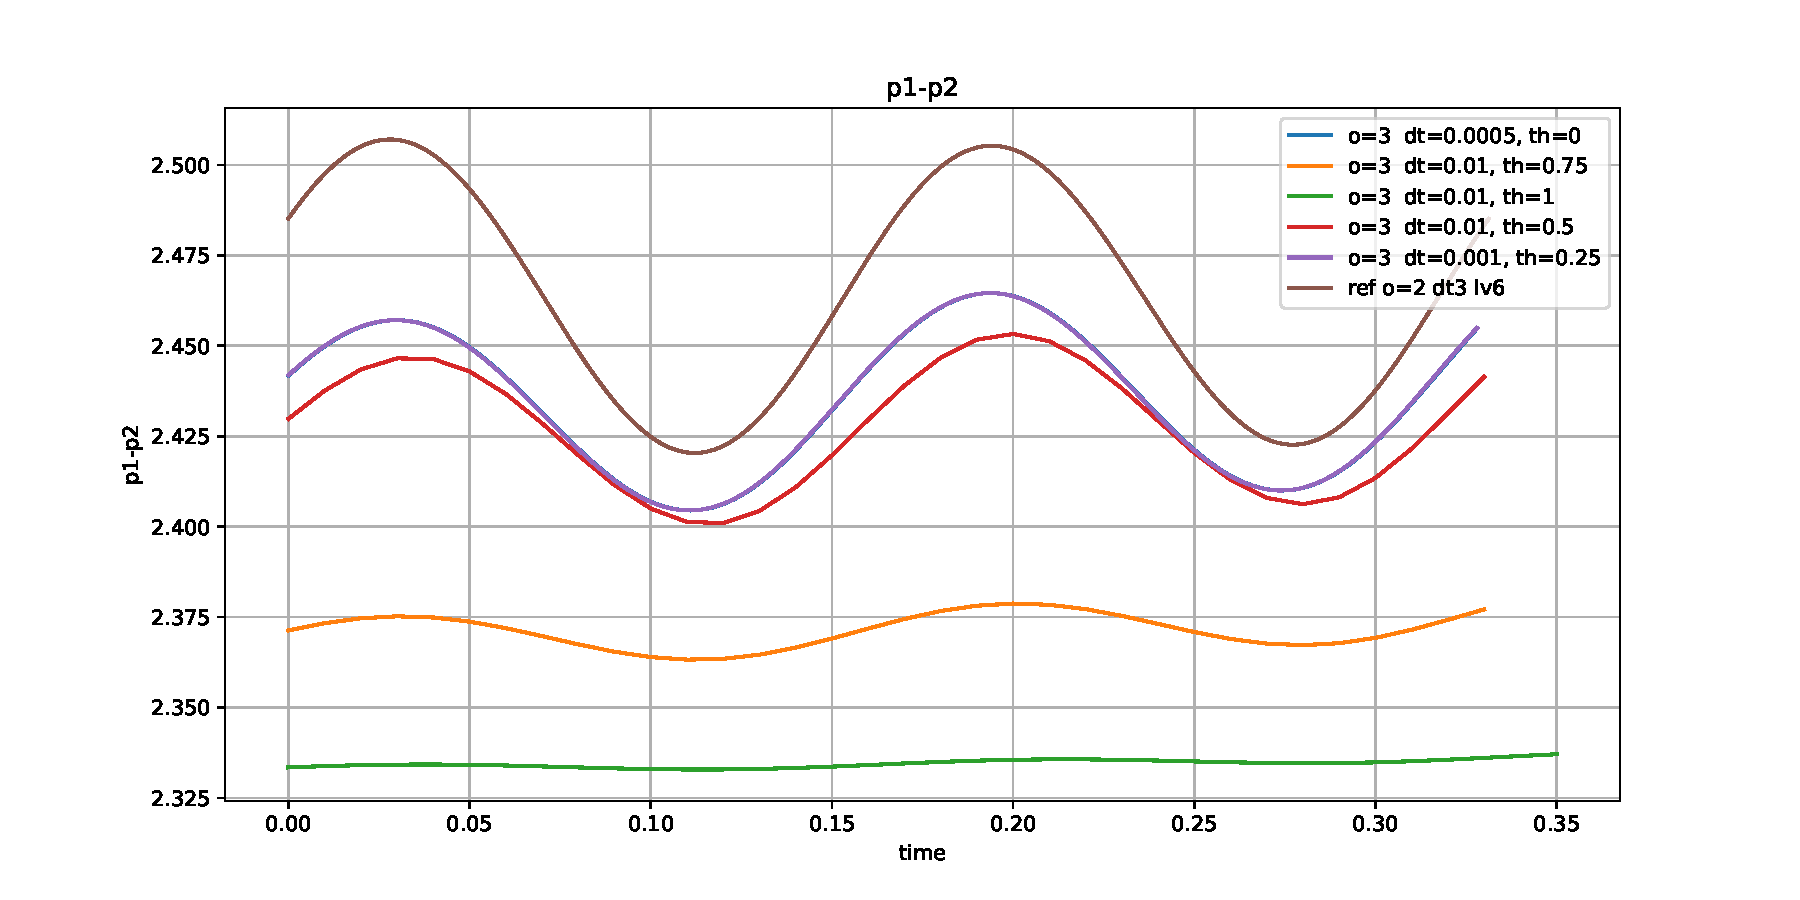
\includegraphics[width=0.75\columnwidth]{p1p2_theta}

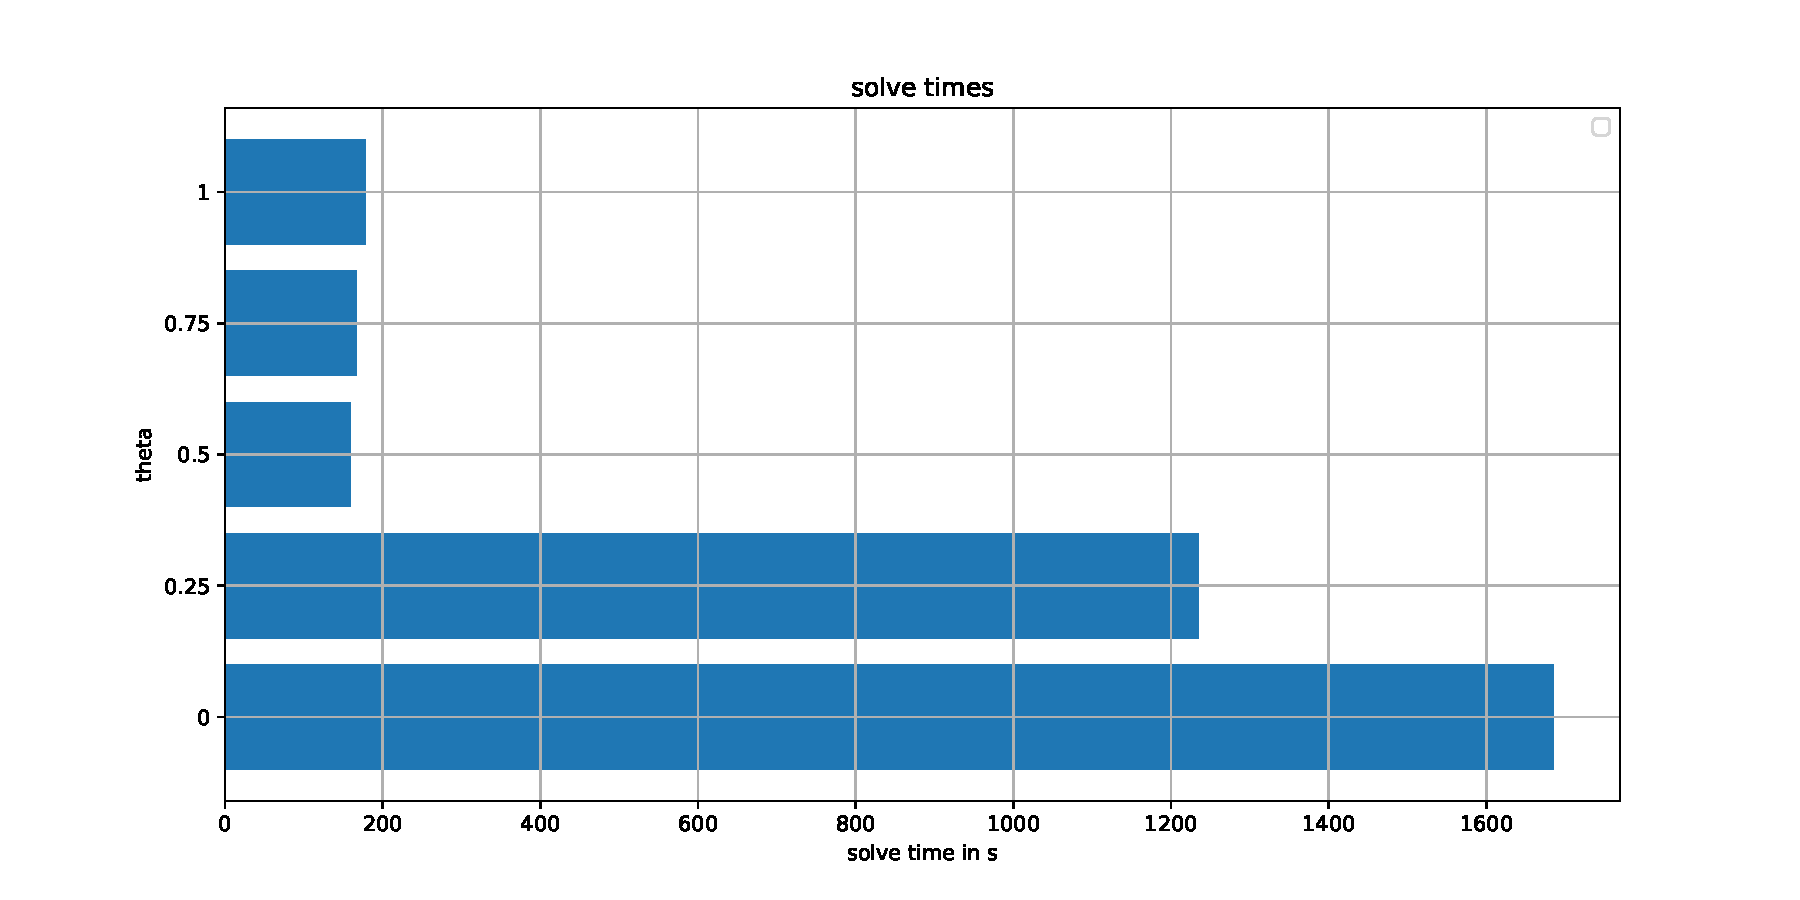
\includegraphics[width=0.75\columnwidth]{solve_times_theta}


\subsection{Comparing $\theta\geq 0.5$ methods for $t\in[0,5]$}

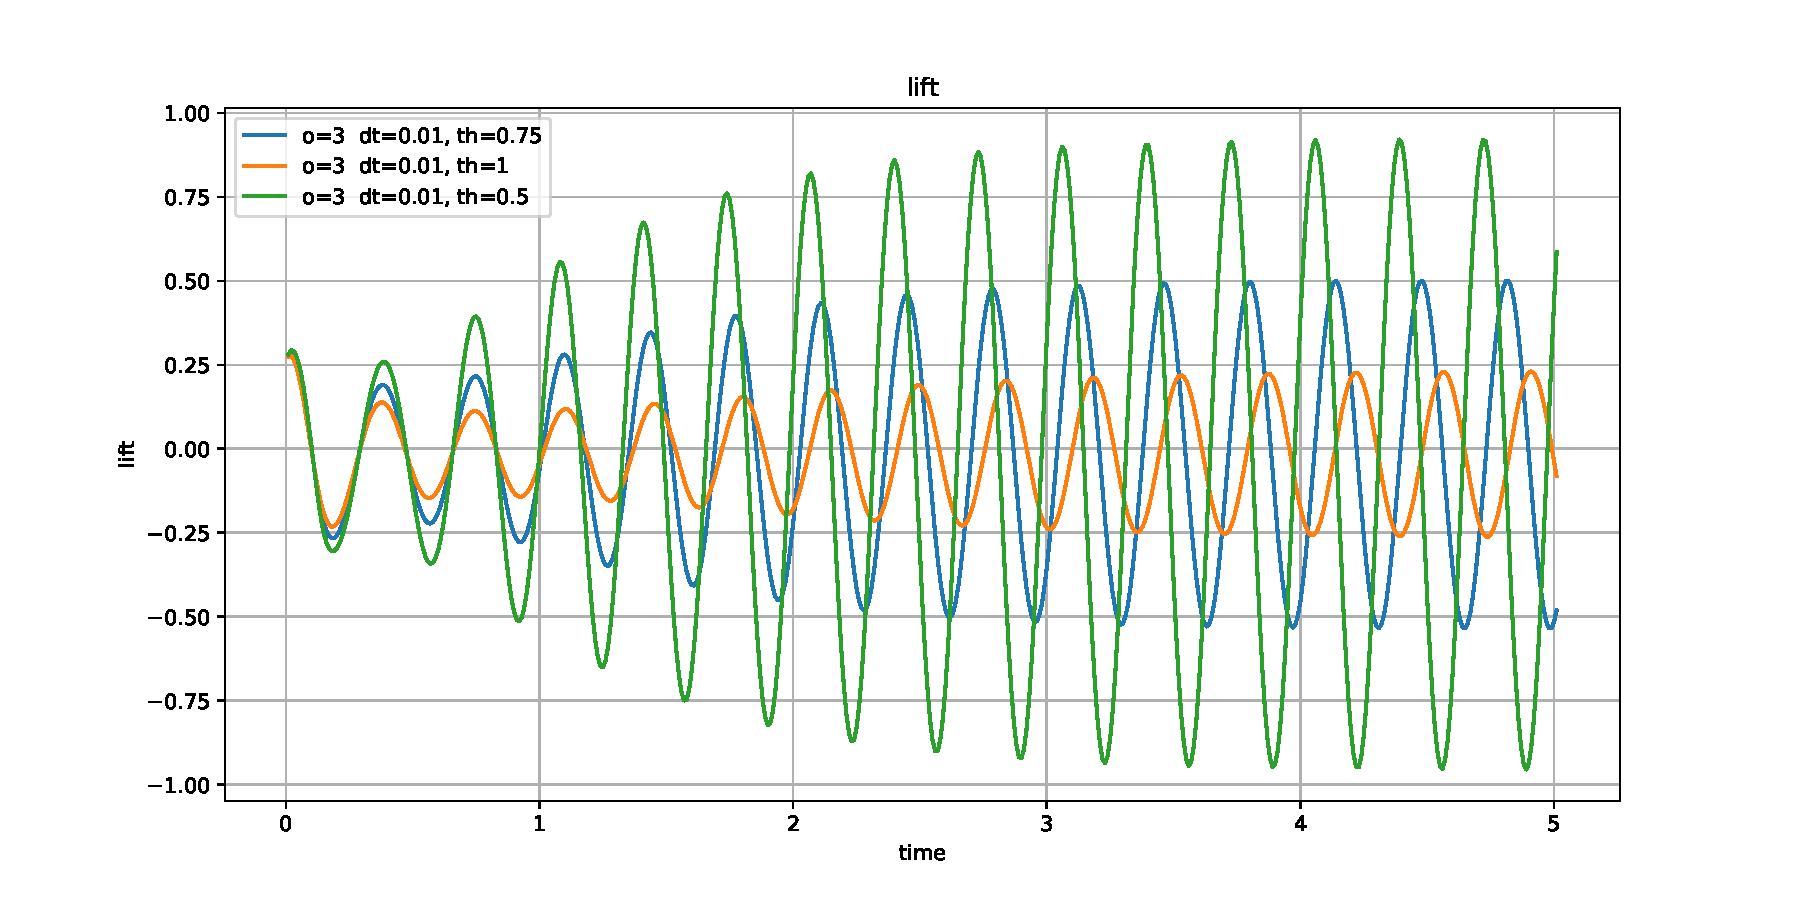
\includegraphics[width=0.75\columnwidth]{lift_full_implicit}

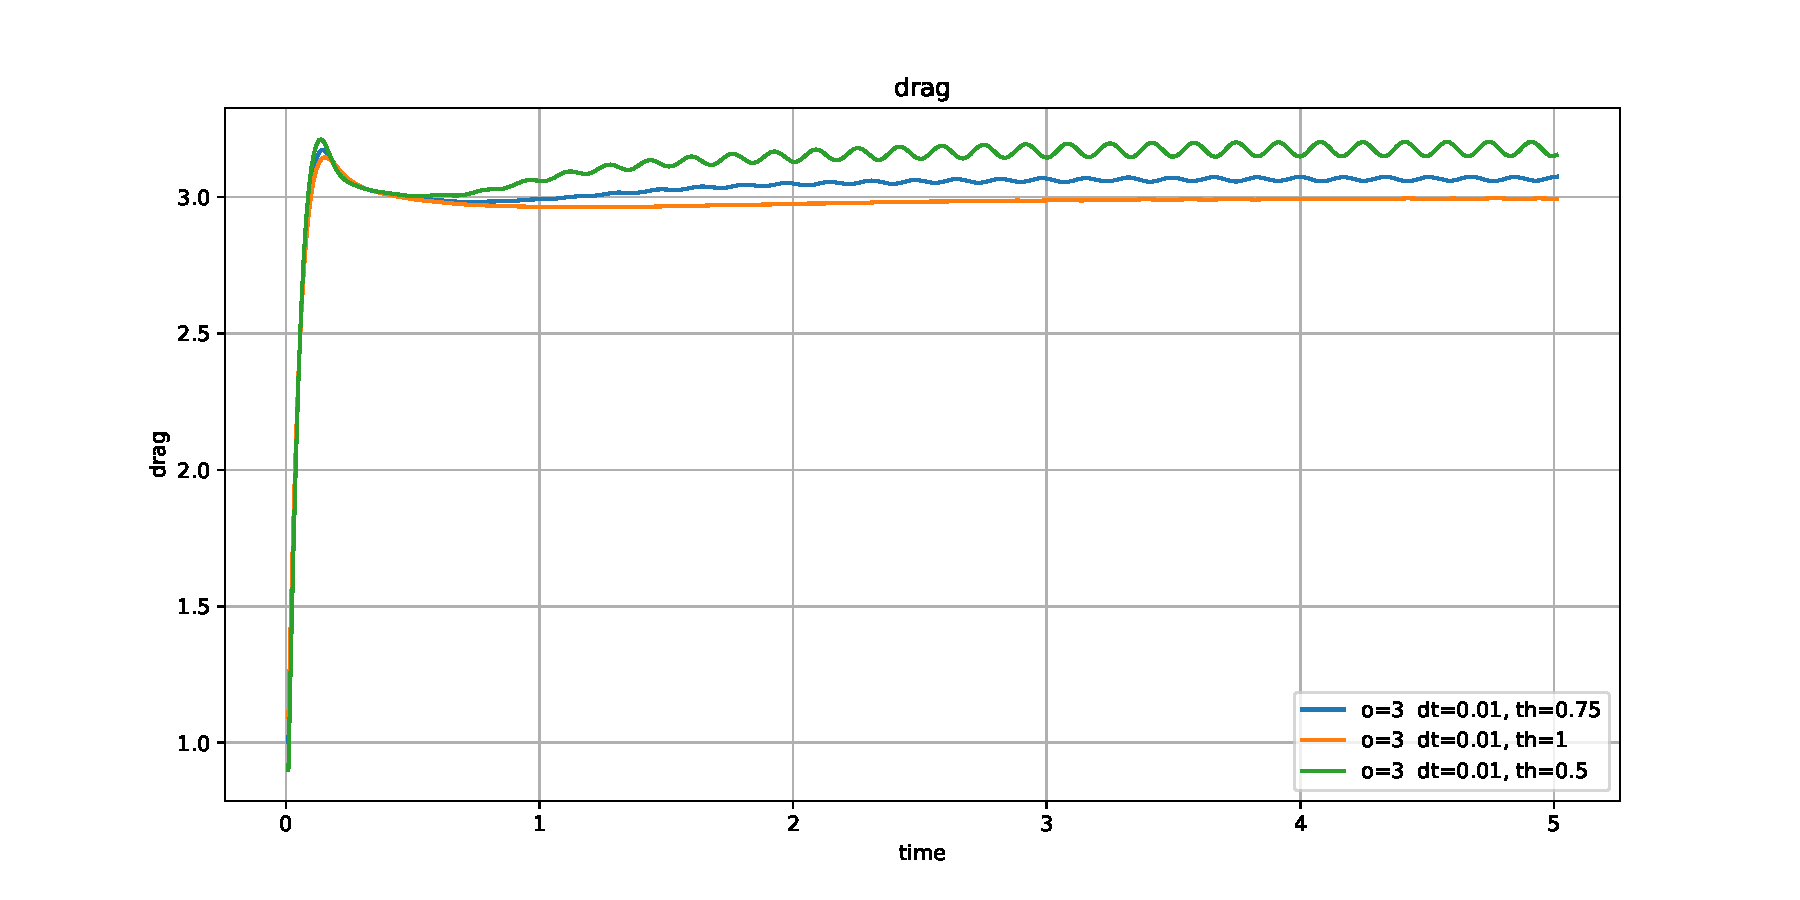
\includegraphics[width=0.75\columnwidth]{drag_full_implicit}

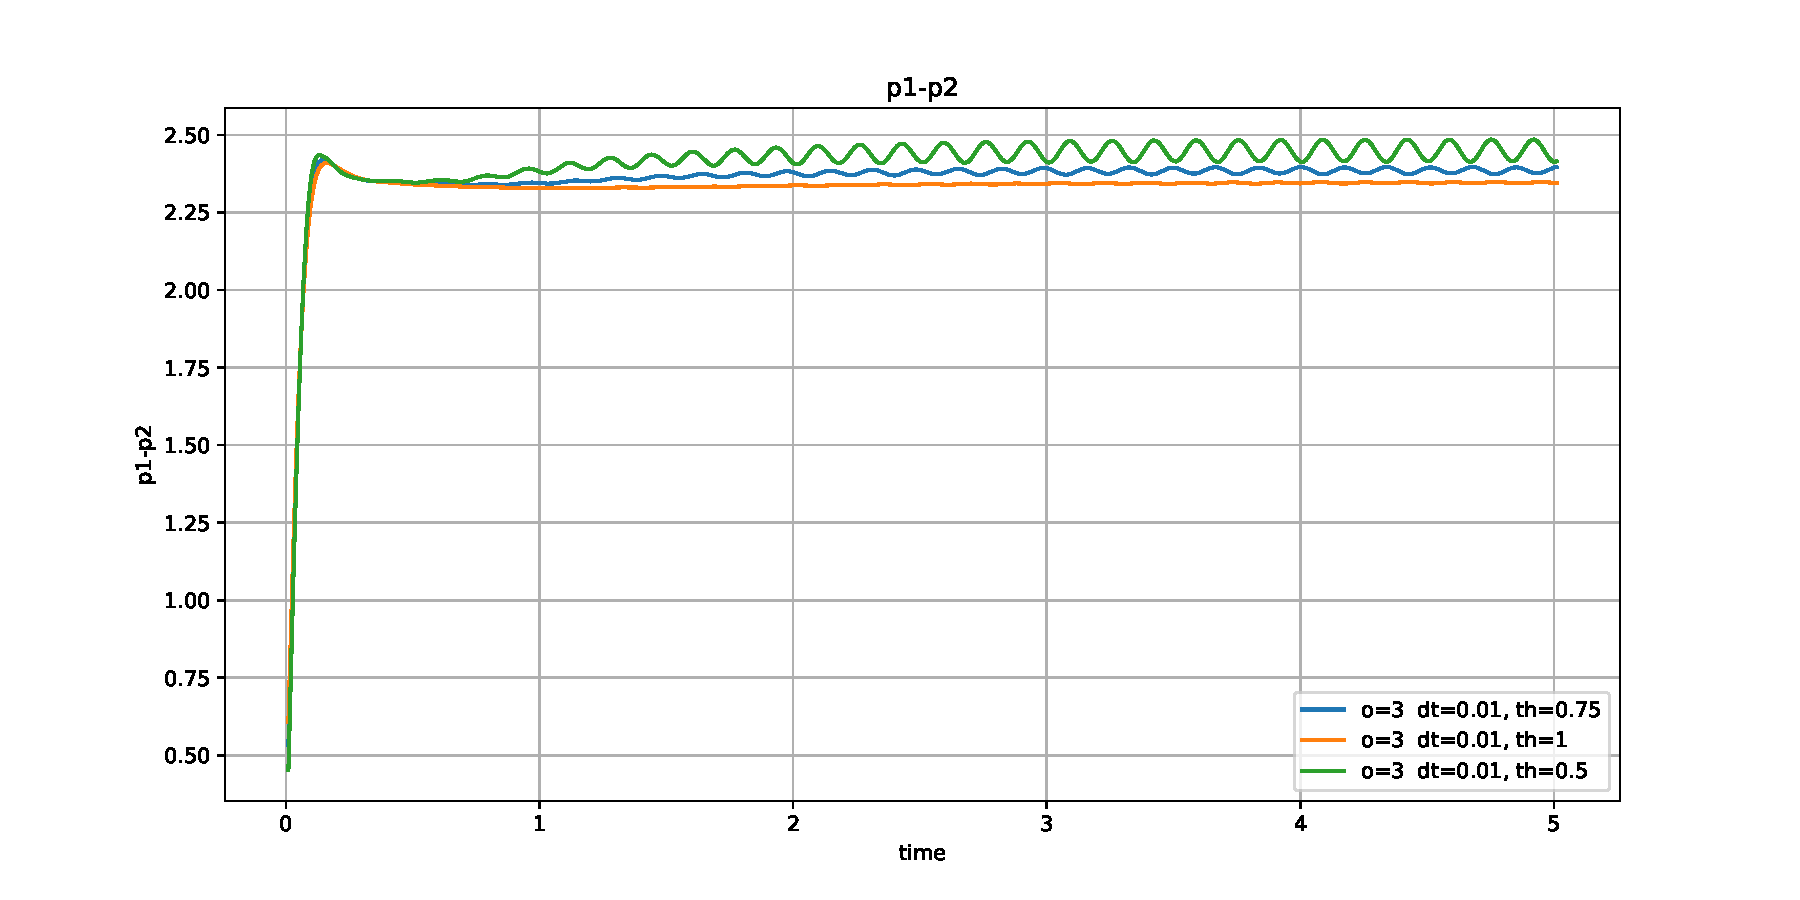
\includegraphics[width=0.75\columnwidth]{p1p2_full_implicit}

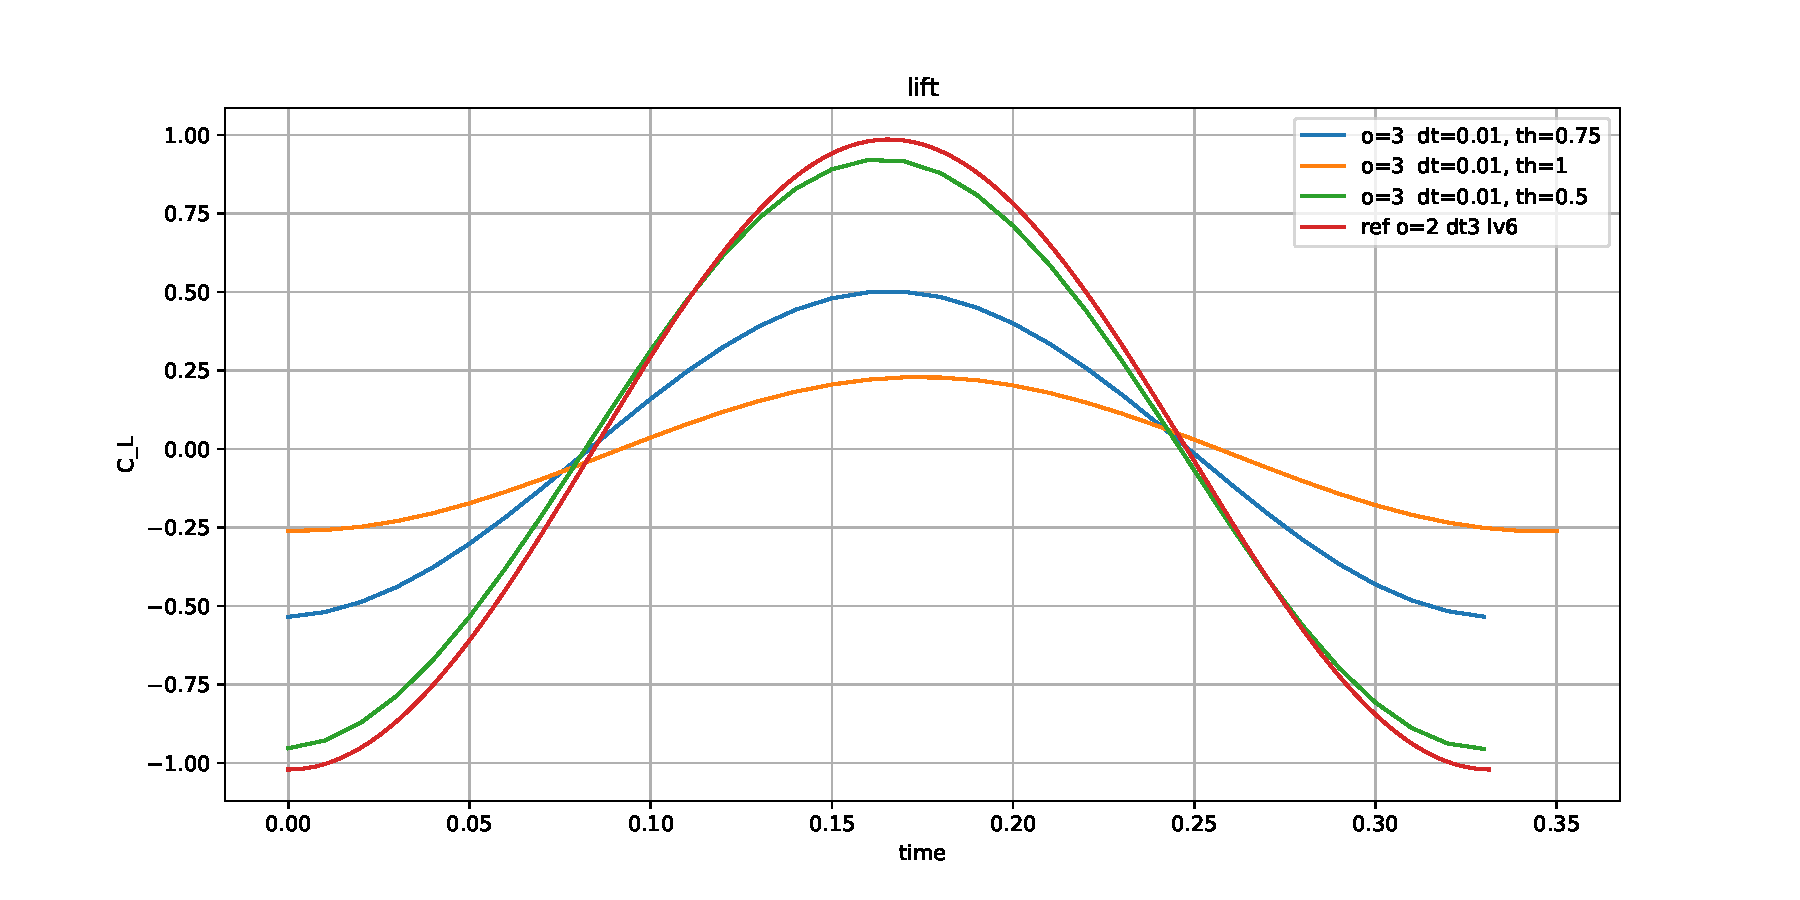
\includegraphics[width=0.75\columnwidth]{lift_full_implicit_per}

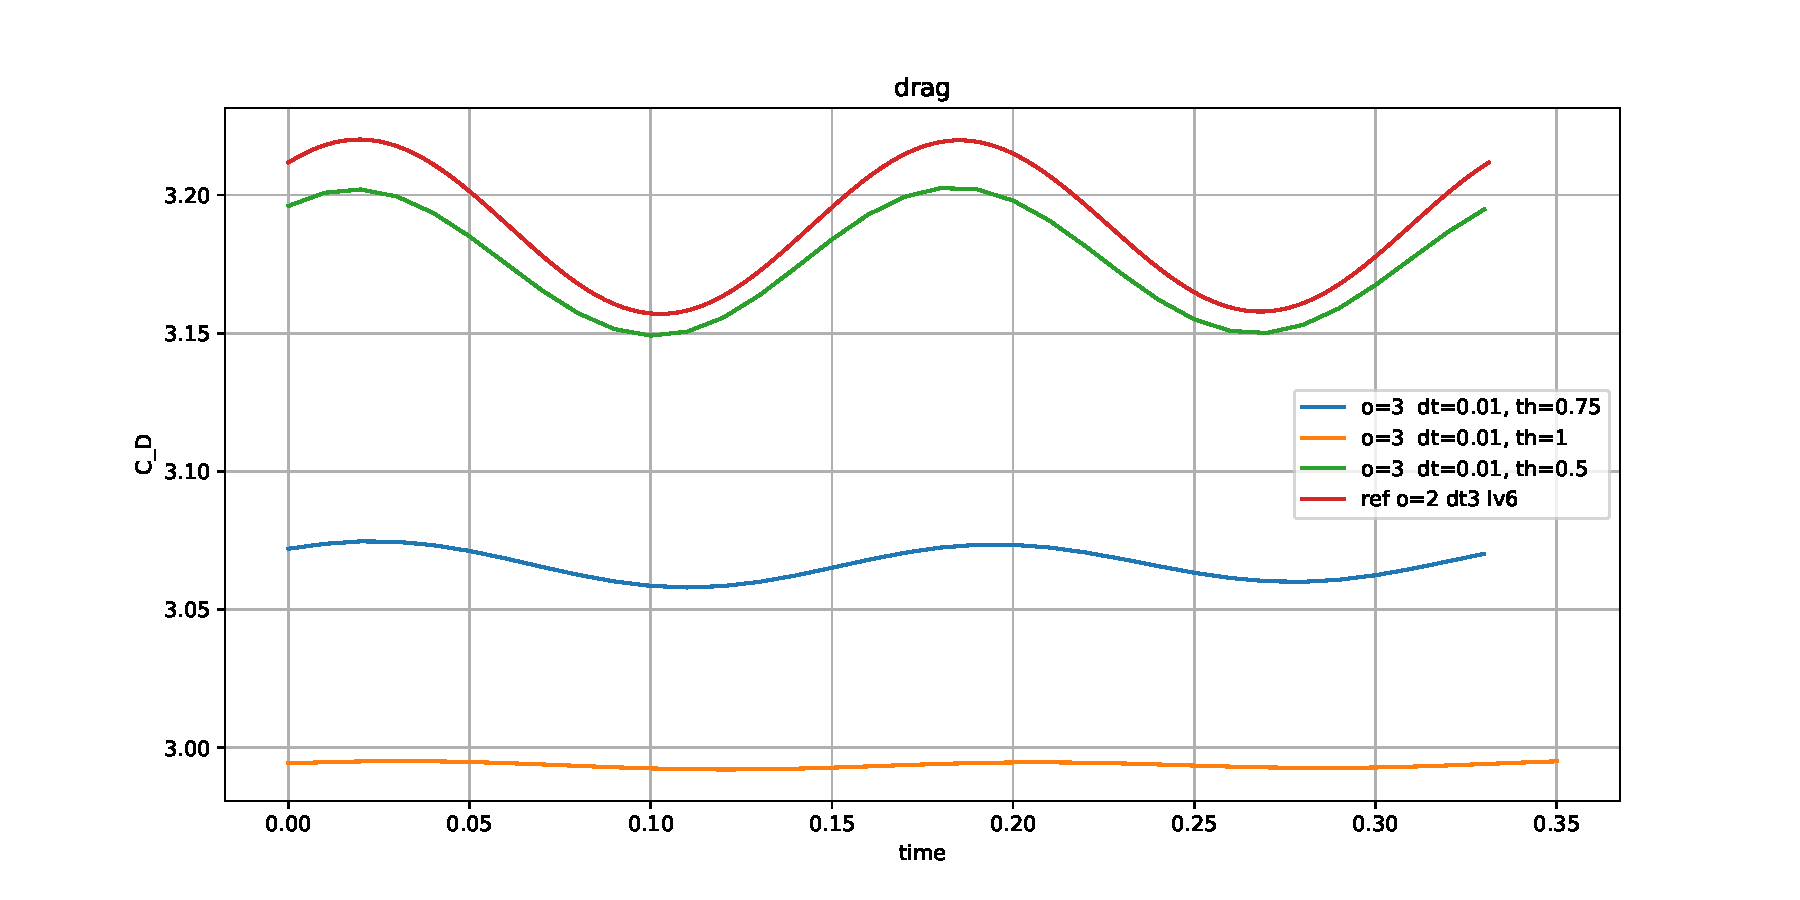
\includegraphics[width=0.75\columnwidth]{drag_full_implicit_per}

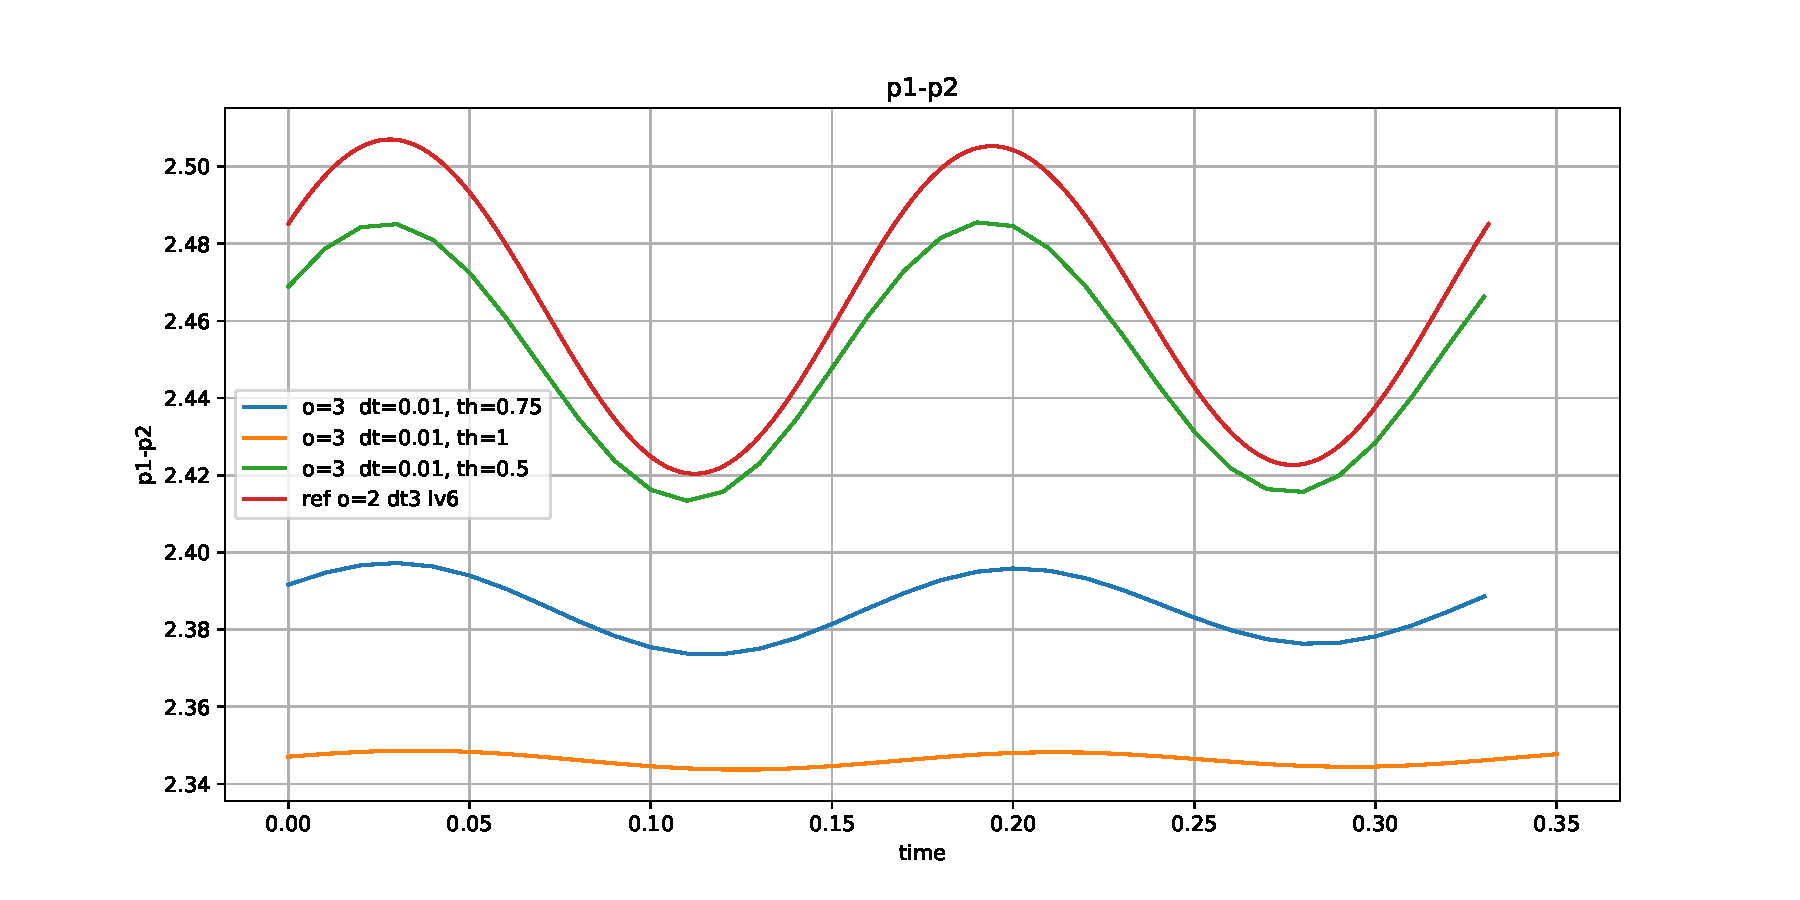
\includegraphics[width=0.75\columnwidth]{p1p2_full_implicit_per}


\subsection{p-refinement at $\theta= 0.5$ method for $t\in[0,5]$}

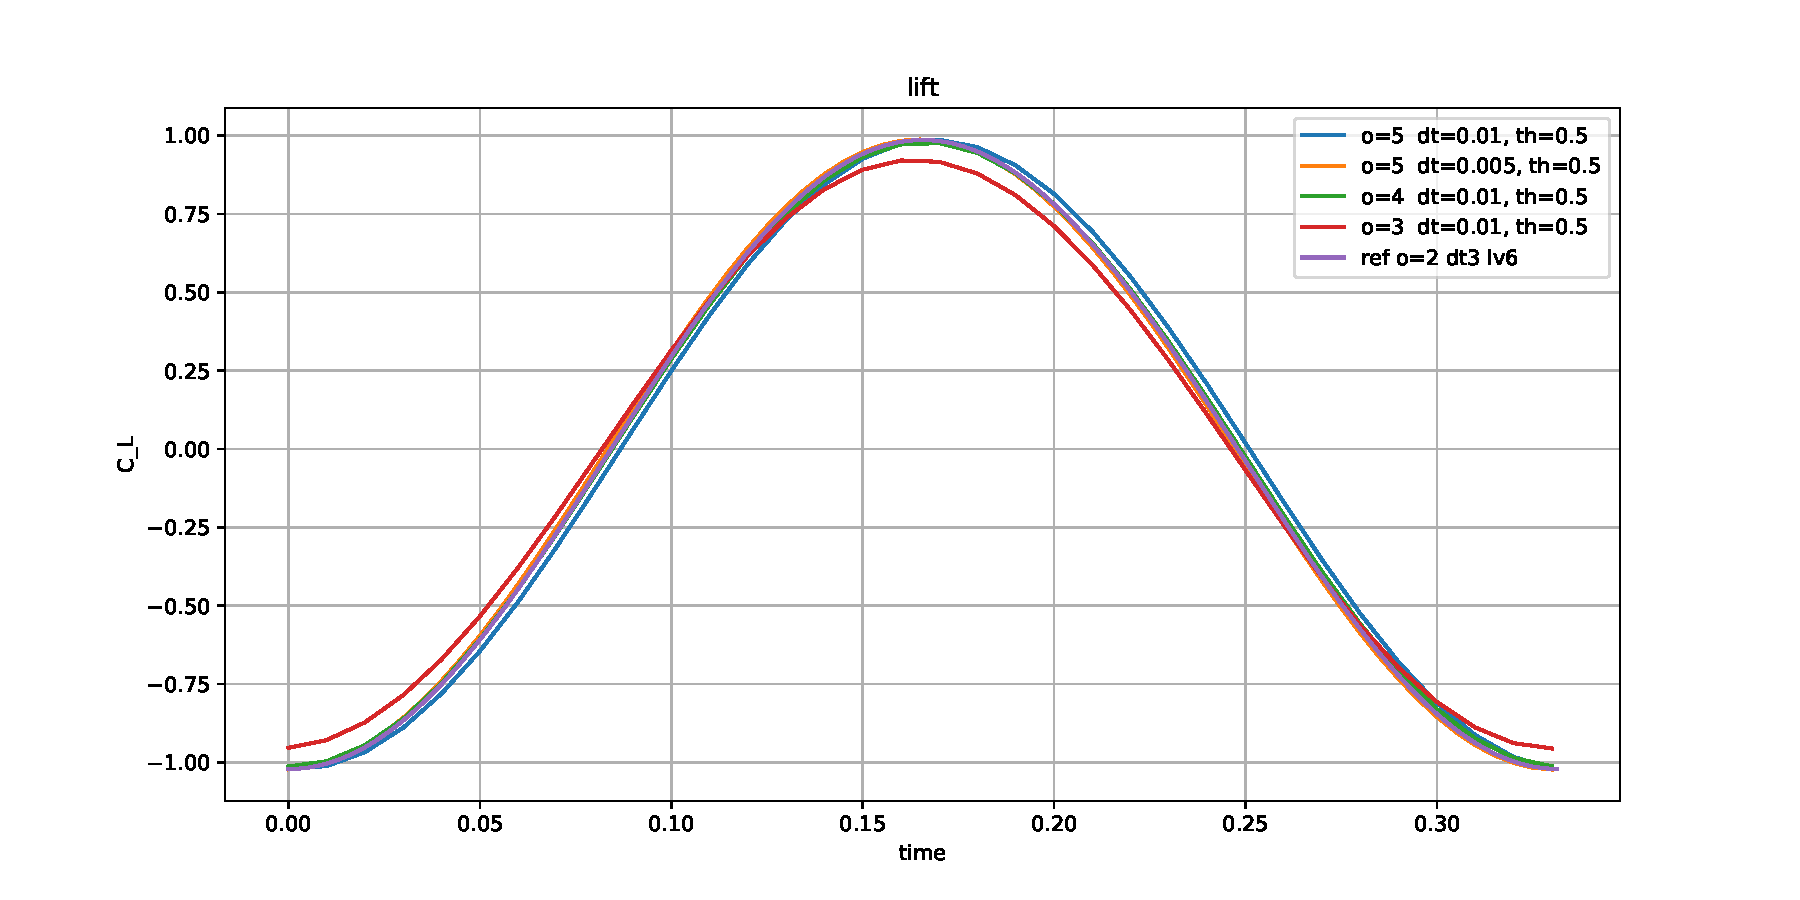
\includegraphics[width=0.75\columnwidth]{lift_final}

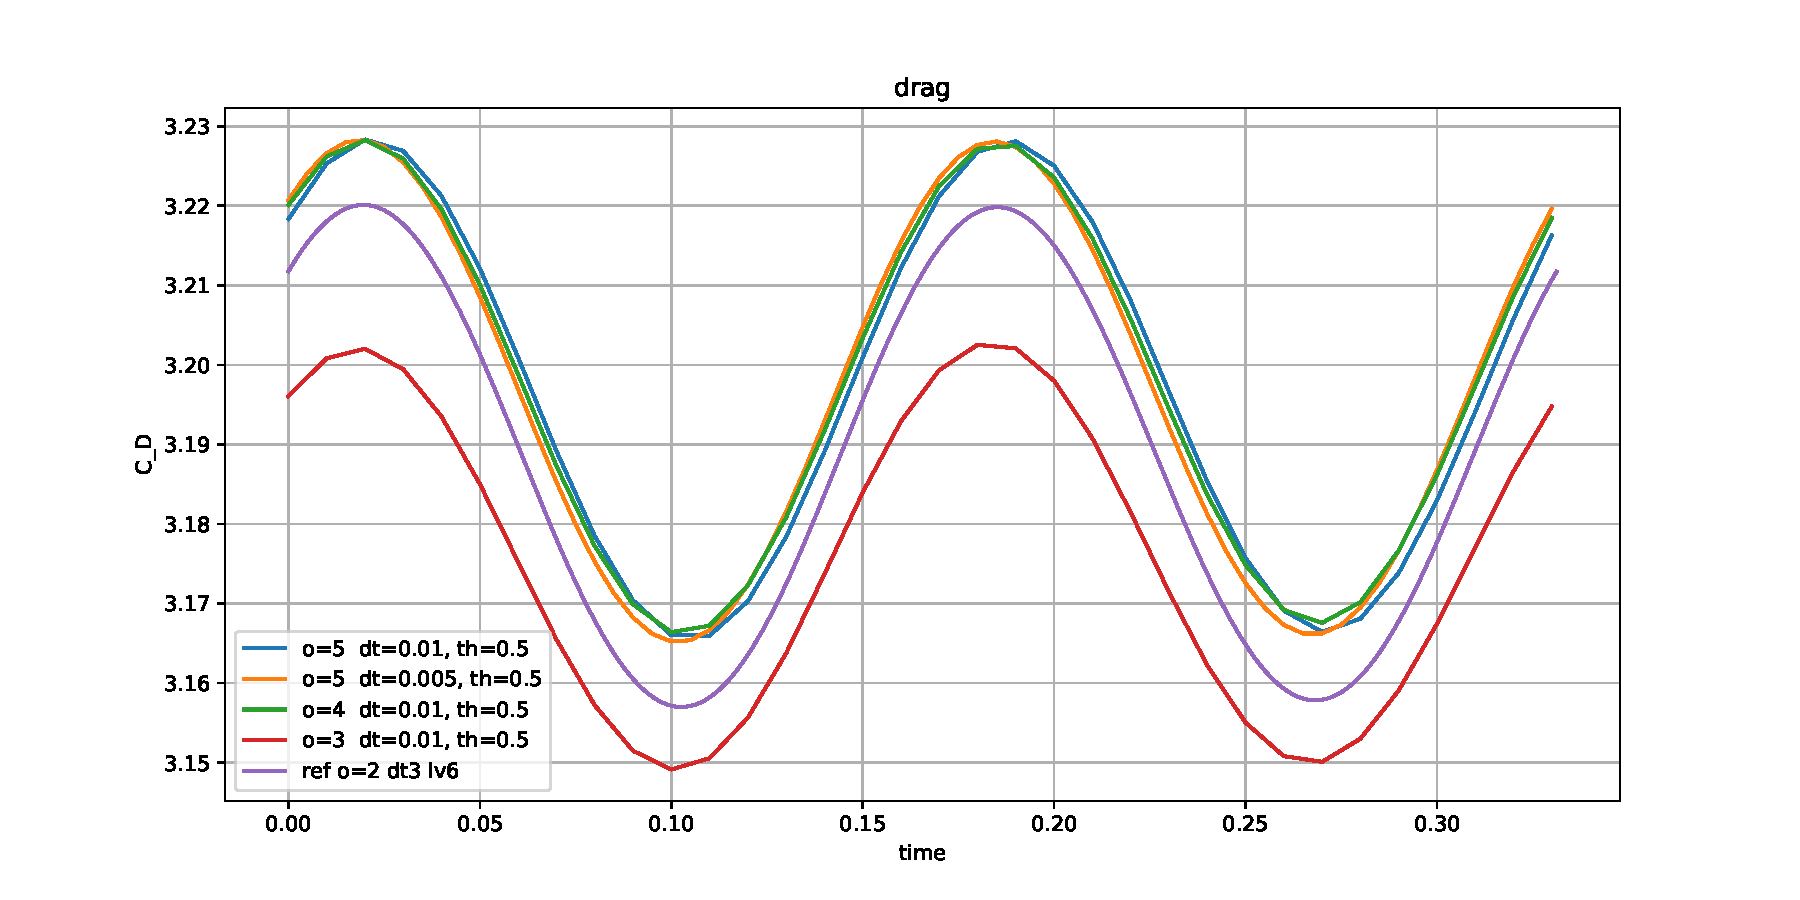
\includegraphics[width=0.75\columnwidth]{drag_final}

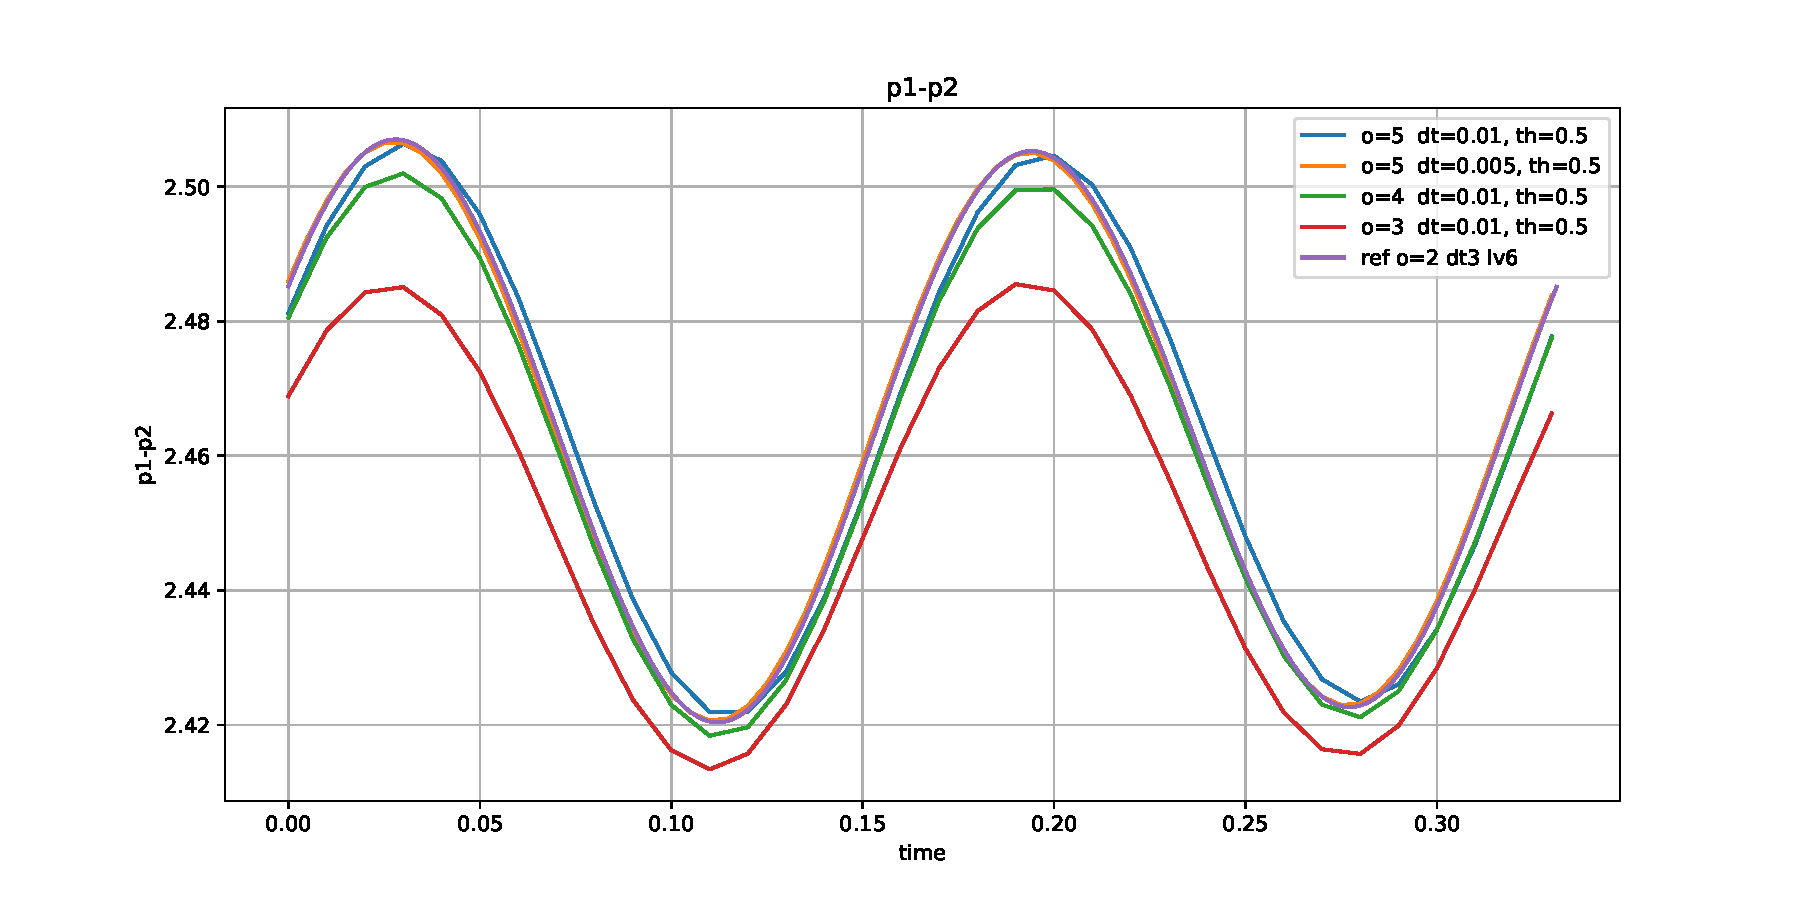
\includegraphics[width=0.75\columnwidth]{p1p2_final}



%Bibliography
\newpage
\bibliographystyle{plain}
\bibliography{Biblothek}

\end{document}
